\section{ Implementation and Used Technologies}
\phantomsection

For a better understanding of the application, on how it works, how it behaves for the patient and in general for those who will use it, it is better and I would say important to describe the technologies that were used to build Kyno. In this chapter will be analysed the implementation of the features that presents the Kyno as a software, will be shown some code samples and analysed the solutions that were choosed to develop the application.

\subsection{System Requirements}
In order to run the application and to have a nice user experience, there is needed for the client to have 2 componenets.

\begin{itemize}
\item A computer, laptop or any system/device where you can install a desktop application

\item A Leap Motion tracking device with again the ability to install software on your device.
\end{itemize}

As we can see the requirements are not that simple and easy to get since the Leap Motion can be bought only online from USA and cost almost 100 euros. However the application will come with the Leap Motion controller in the set.

\subsection {Technologies Used}
\subsubsection {Unity}
Unity is a powerful cross-platform 3D engine and a user friendly development environment. Easy enough for the beginner and powerful enough for the expert.
\\
\textbf{Why Unity over others?}

The main "pro" of Unty is that it's crazy fast. I'm not talking about performance here, but about development speed. It has:

\begin{itemize}
\item \textbf{Unified asset pipeline}. No need to spend time on resource subsystem at all, no buggy import routines to write and fix: just drop a file into folder, and it works.
\item \textbf{Integrated level editor}. No need to spend time on level tools: just get straight to business.

\item \textbf{Great tweaking and debugging support}.All your scripting variables are shown in the editor right as you play, and can be changed on the fly too - and all this without writing a single line of code. Pause the application anytime, or step through code one statement at a time.

\item \textbf{Quite comprehesive library of ready-made components}. Rendering, sound, physics, controls - a lot of "boilerplate" code is already written so that you can focus on the application and not on how to create an engine.
\end{itemize}

One aspect is that Unity is a game engine and editor that publishes almost anywhere. What does it mean “everywhere”? One can divide the game world in four continents: consoles, smartphones, desktop (installed), browser.  Unity runs in most “countries” from all these continents – as shown in \mbox{figure \ref{everywhere}}.
\begin{figure}[!h]
\centering
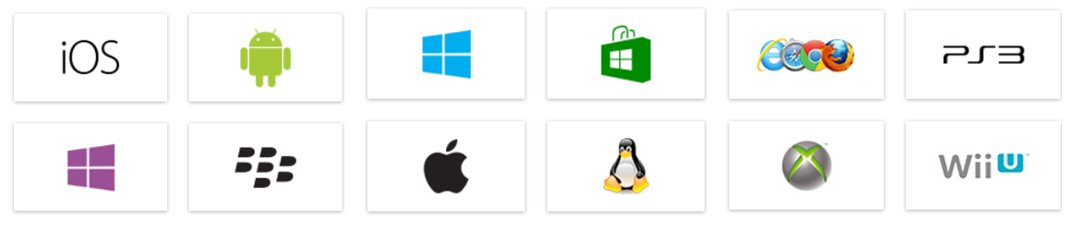
\includegraphics[ width = 14cm]{everywhere}
\caption{Exercising state diagram \cite{multiplatform}}\label{everywhere}
\end{figure}

Application created in Unity can be deployed into multiple platforms simply by downloading and installing support of these platform. After that offcourse by changing your code so that it will work on other platform too.

So let's see 2 examples in of how Unity handles a mouse input in a desktop application and fingers input in a mobile application.
\begin{lstlisting}[caption={Mouse input for desktop application in Unity \cite{mousedown}.},label={mouseInput}]
 void Update() {
         if (Input.GetMouseButtonDown(0))
             Debug.Log("Pressed left click.");
         
         if (Input.GetMouseButtonDown(1))
             Debug.Log("Pressed right click.");
         
         if (Input.GetMouseButtonDown(2))
             Debug.Log("Pressed middle click.");
         
     }
\end{lstlisting}

As we can see \autoref{mouseInput}  returns true during the frame the user pressed the given mouse button. Either will be left click, middle or right click.

\begin{lstlisting}[caption={Multiple touch input for mobile application in Unity \cite{multipletouch}.},label={touchInput}]
void Update () 
    {
        Touch myTouch = Input.GetTouch(0);
        Touch[] myTouches = Input.touches;
        for(int i = 0; i < Input.touchCount; i++)
        {
            //Do something with the touches
        }
    }
\end{lstlisting}

In \autoref{touchInput} Unity handles multi-touch by giving you the number of touches on the screen during a given frame, and/or gives you an array of all touches during a frame. While myTouch will be the first touch the user did and myTouches will be the total amount of touches the user does.

This way Unity does for every platform, it is a console, it is a desktop computer, a mobile phone or web browser. Unity make life easire.
\subsubsection {Leap Motion}



www.notebookcheck.net/Review-Leap-Motion-Motion-Control-Technology.98821.0.html
\subsubsection {C\# or JavaScript?}

Mono as a script host. While one can argue about merits of C\# as a language, Mono's base class library offers a wealth of functions. Collections, I/O, multithreading, and insanely expressive LINQ all speed up development considerably.
Also, Unity3d is really good on multiple platforms. Of course, you can't create, say, a windows .exe game and then magically have it "just work" on the iPhone; but Unity gets pretty close to that. What is required is "tweaking" more than "porting".
\subsubsection {Leap Motion SDK}
\subsubsection {LitJson}
\subsubsection{APIs}
\subsubsection{Leap Motion API}

\subsection{Implementation}
\subsubsection{Software license}
Kyno will be offered for a period of 1 month for free. In this period, the software will be tested and feedback will be prompted from users. It is very important at this stage to see how the application is doing, where are the problems, what features need to be added. 

After 1 month of free using, a monthly or yearly subscription plan will be applied with different prices for individual patients or hospitals and rehabilitation centers.

 \autoref{bootstrap}. This simple structure makes it easy to locate the files and edit them when it's needed.
\begin{lstlisting}[caption={Bootstrap folder structure},label={createController}]
  protected virtual void Start() {
      createController();
    }
    
protected void createController() {
      if (leap_controller_ != null) {
        destroyController();
      }

      leap_controller_ = new Controller();
      leap_controller_.Device += onHandControllerConnect;
    }
    
    protected void destroyController() {
      if (leap_controller_ != null) {
        if (leap_controller_.IsConnected) {
          leap_controller_.ClearPolicy(Controller.PolicyFlag.POLICY_OPTIMIZE_HMD);
        }
        leap_controller_.StopConnection();
        leap_controller_ = null;
      }
    }

    protected void onHandControllerConnect(object sender, LeapEventArgs args) {
      leap_controller_.Device -= onHandControllerConnect;
    }
\end{lstlisting}
\clearpage